\chapter{撰写要求}

\section{论文正文}
\subsection{图标等编号}

论文中的图、表、附注、公式、算式等,一律用阿拉伯数字分章依序连续编码。其标注形式
应便于互相区别,如:图1-1(第1章第一个图)、图2-2(第2章第二个图);表3-2(第3章
第二个表)等。附录的图表参考正文的编号方式,如附图1-1或附表1-1。

\subsection{图和表}

论文中若有图和表,应设置图表目录,先列图后列表,置于目录页后,另页编排。

\subsubsection{图}

图片大小适当,图边界在页面范围内(图边界离页面边界距离大于页边距)。若图片中包含
文字,文字大小不超过正文文字大小。\\
图包括曲线图、构造图、示意图、框图、流程图、记录图、地图、照片等,宜插入正文适当
位置。引用的图必须注明来源。具体要求如下:
\begin{itemize}
    \item 图应具有“自明性”,即只看图、图题和图注,不阅读正文,就可理解图意。每一图应有简短确切的图题,连同图序置于图下居中。
    \item 图中的符号标记、代码及实验条件等,可用最简练的文字横排于图框内或图框外的某一部位作为图注说明,全文统一。图题建议用中文及英文两种文字表达。
    \item 照片图要求主要显示部分的轮廓鲜明,便于制版,如用放大、缩小的复制品,必须清晰,反差适中,照片上应有表示目的物尺寸的标尺。
\end{itemize}

\section{功能介绍}

\subsection{数学公式}

比如\autoref{eq:1}
\begin{equation}
    \label{eq:1}
    \int_{-\infty}^{+\infty} e^{-x^2} dx = \sqrt{\pi}
\end{equation}

\subsection{图片}

比如\autoref{fig:pngtest}. 注意模板中已经默认设置figure及table环境的位置参数为\verb|htbp|, 不能再单独设置.
\begin{figure}
    \centering
    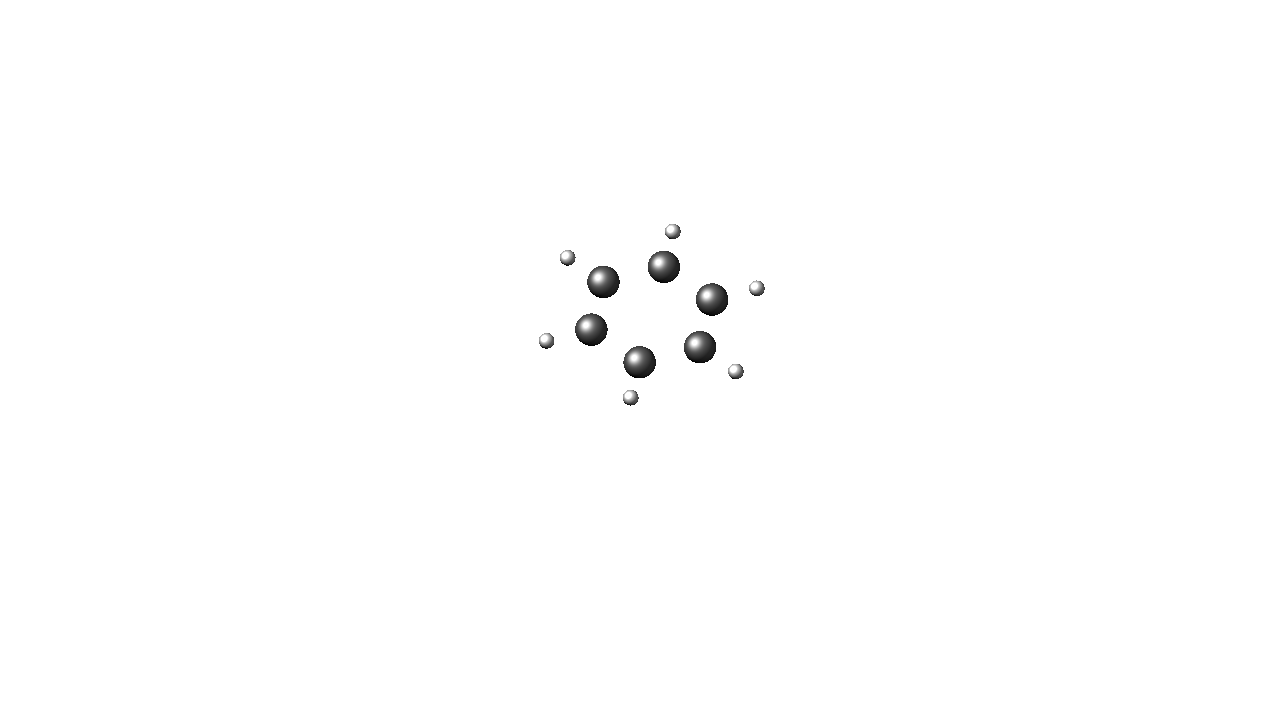
\includegraphics[width=0.5\textwidth]{pngtest}
    \bicaption{ucasthesis 图片测试}{ucasthesis figure test}\label{fig:pngtest}
\end{figure}

\subsection{表格}

请见\autoref{tab:sample}。
\begin{table}
    \bicaption{这是一个样表}{This is a sample table}\label{tab:sample}
    \centering
    \setlength{\tabcolsep}{4pt}% column separation
    \renewcommand{\arraystretch}{1.2}%row space
    \begin{tabular}{lcccccccc}
        \toprule
        行号 & \multicolumn{8}{c}{跨多列的标题}\\
        %\cline{2-9}% partial hline from column i to column j
        \midrule
        Row 1 & 1 & 2 & 3 & 6 & 7 & 8 \\
        Row 2 & 1 & 2 & 3 & 6 & 7 & 8 \\
        Row 3 & 1 & 2 & 3 & 6 & 7 & 8 \\
        Row 4 & 1 & 2 & 3 & 6 & 7 & 8 \\
        \bottomrule
    \end{tabular}
\end{table}

\subsection{术语}

有符号: \gls{pi}, 有缩写: \gls{spi}, 都可以.

\subsection{引用}
本模板使用biber进行文献编译,基本符合2015国标的参考文献格式。默认情况下,按照国
科大的指导标准,使用数字顺序的引用方式没有严格限制,这也是最方便的引用途径。 如
果您一定要使用作者年份制引用,请参照参考文献模板的说明进行使用。看看这个例子,关
于书的\cite{tex, companion, ColdSources},还有这些\cite{Krasnogor2004e, clzs,
zjsw},关于杂志的\cite{ELIDRISSI94, MELLINGER96, SHELL02},硕士论文\cite{zhubajie, metamori2004},
博士论文\cite{shaheshang, FistSystem01},标准文件\cite{IEEE-1363},
会议论文\cite{DPMG,kocher99},技术报告\cite{NPB2}。中文参考文
献\cite{cnarticle}应增加 \texttt{lang=``zh''} 字段,以便进行相应处理。更多参考文
献模板使用方法请参照参考文献模板作者说明
\url{https://github.com/hushidong/biblatex-gb7714-2015}。

\subsection{代码}

代码可以是行内的, 如\mintinline{python3}{print('是字符串' if isinstance(aString, str) else '不是字符串')}, 可以是单行的:
\mint{tex}{\inputminted[firstline=16, lastline=37]{c}{assets/example.c}}
也可以是如下从指定文件指定范围插入的代码块\autoref{code:sample}。
\begin{listing}[H]
    \inputminted[firstline=16, lastline=37]{c}{assets/example.c}
    \bicaption{这是一段示例代码}{A sample code}\label{code:sample}
\end{listing}

\subsection{算法}

这有一个\autoref{alg:alg1}

\begin{algorithm}
    \caption{Calculate \(y = x^n$}\label{alg:alg1}
    \begin{algorithmic}
        % 输入
        \REQUIRE \(n \geq 0 \vee x \neq 0\)
        % 输出
        \ENSURE \(y = x^n\)

        % 初始化
        \STATE \(y \leftarrow 1\)

        % 逻辑
        \IF{\(n < 0\)}
        \STATE \(X \leftarrow 1 / x\)
        \STATE \(N \leftarrow -n\)
        \ELSE
        \STATE \(X \leftarrow x\)
        \STATE \(N \leftarrow n\)
        \ENDIF

        \WHILE{\(N \neq 0\)}
        \IF{\(N\) is even}
        \STATE \(X \leftarrow X \times X\)
        \STATE \(N \leftarrow N / 2\)
        \ELSIF{\(N\) is odd}
        \STATE \(y \leftarrow y \times X\)
        \STATE \(N \leftarrow N - 1\)
        \ENDIF
        \ENDWHILE
    \end{algorithmic}
\end{algorithm}
